% IF YOU CAN SEE THIS GO CONTRIBUTE >:(

\documentclass[letterpaper, 8pt]{extarticle}
\usepackage{amssymb,amsmath,amsthm,amsfonts}
\usepackage{multicol,multirow}
\usepackage{calc}
\usepackage{ifthen}
\usepackage[landscape]{geometry}
\usepackage[colorlinks=true,citecolor=blue,linkcolor=blue]{hyperref}

\usepackage{booktabs}
\usepackage{ulem}
\usepackage{enumitem}
\usepackage{tabulary}
\usepackage{graphicx}
\usepackage{siunitx}
\usepackage{tikz}
\usepackage{derivative}
\usepackage{svg}
\usepackage{listings}
\usepackage{setspace}
\usepackage{listings}
\usepackage{xcolor}
\usepackage{courier}
\usepackage{syntax}
\usepackage{mathpartir}
\usepackage{siunitx}
\usepackage{tabularx}

% minimal line spacing
% \setstretch{0.1}

% set borders (experimentally determined to minimize cutoff and
% maximize space on school printers)
\geometry{top=.25in,left=.25in,right=.25in,bottom=.35in}

% make figures work better in multicol
\newenvironment{Figure}
{\par\medskip\noindent\minipage}
{\endminipage\par\medskip}

\pagestyle{empty} % clear page

% rewrite section commands to be smaller
\makeatletter
\renewcommand{\section}{\@startsection{section}{1}{0mm}%
  {-1explus -.5ex minus -.2ex}%
  {0.5ex plus .2ex}%x
{\normalfont\small\bfseries}}
\renewcommand{\subsection}{\@startsection{subsection}{2}{0mm}%
  {-1explus -.5ex minus -.2ex}%
  {0.5ex plus .2ex}%
{\normalfont\tiny\bfseries}}
\renewcommand{\subsubsection}{\@startsection{subsubsection}{3}{0mm}%
  {-1ex plus -.5ex minus -.2ex}%
  {1ex plus .2ex}%
{\normalfont\tiny\bfseries\itshape}}
\makeatother
\setcounter{secnumdepth}{0} % disable section numbering

% disable indenting
\setlength{\parindent}{0pt}
\setlength{\parskip}{0pt plus 0.5ex}

% Custom siunitx defs
\DeclareSIUnit\noop{\relax}
\NewDocumentCommand\prefixvalue{m}{%
  \qty[prefix-mode=extract-exponent,print-unity-mantissa=false]{1}{#1\noop}
}

% Shorthand definitions
\newcommand{\To}{\Rightarrow}
\newcommand{\ttt}{\texttt}
\newcommand{\ra}{\rightarrow}

% condense itemize & enumerate
\let\olditemize=\itemize \let\endolditemize=\enditemize
\renewenvironment{itemize}{\olditemize \itemsep0em}{\endolditemize}
\let\oldenumerate=\enumerate \let\endoldenumerate=\endenumerate
\renewenvironment{enumerate}{\oldenumerate \itemsep0em}{\endoldenumerate}
\setlist[itemize]{noitemsep, topsep=0pt, leftmargin=*}
\setlist[enumerate]{noitemsep, topsep=0pt, leftmargin=*}

% sarah's q and a commands
\newcommand{\question}[1]{{ \scriptsize \color{blue}{#1}}}
\newcommand{\answer}[1]{{ \scriptsize {#1}}}

\title{3GC3}

\begin{document}
\raggedright
\tiny

% make listings look nicer
\lstset{
  tabsize = 2, %% set tab space width
  showstringspaces = false, %% prevent space marking in strings,
  % string is defined as the text that is generally printed directly
  % to the console
  basicstyle = \tiny\ttfamily, %% set listing font and size
  breaklines = true, %% enable line breaking
  numberstyle = \tiny,
  postbreak = \mbox{\textcolor{red}{\(\hookrightarrow\)}\space}
}

\begin{center}
  {\textbf{COMPSCI 4NL3 - JOBLESS EDITION}} \\
\end{center}
% set column spacing rules
\setlength{\premulticols}{1pt}
\setlength{\postmulticols}{1pt}
\setlength{\multicolsep}{1pt}
\setlength{\columnsep}{2pt}
\begin{multicols*}{4}
  \section{Regular Expressions}

  \begin{tabularx}{\linewidth}{lX}
    \hline
    Pattern & Matches \\ \hline
    $\backslash s$ & whitespace \\ \hline
    $\backslash d$ & any digit \\ \hline
    $\{N\}$ & exactly \$N\$ of the previous item \\ \hline
    $\backslash w$ & any "word" characters (includes numbers) \\ \hline
    $\backslash S$, $\backslash$D, $\backslash$W & anything NOT in
    the lowercase version of that pattern \\ \hline
    $\backslash b$ & word boundary \\ \hline
    \texttt{\^} & start of the string \\ \hline
    $\$$ & end of the string \\ \hline
    $A|B$ & $A$ or $B$ \\ \hline
    $[a-z]$, $[abcde]$,$[0-9]$ & any character in the brackets of
    specified range of characters \\ \hline
    $.$ & any character \\ \hline
    $?$ & 0 or 1 of the preceding character \\ \hline
    $*$ & 0 or more of the preceding character \\ \hline
    $+$ & 1 or more of the preceding character \\ \hline
    $.*?$ & not greedy \\ \hline
  \end{tabularx}

  \subsection{Example of Not Greedy}

    \begin{lstlisting}
    text = "<tag>I have something here</tag> <tag>but other stuff here</tag>"
    my_regex = r"<tag>.*?<\/tag>"
    re.findall(my_regex, text) = ['<tag>I have something here</tag>', '<tag>but other stuff here</tag>']
    \end{lstlisting}

  \section{Levenshtein Distance}
  \resizebox{0.4\columnwidth}{!}{
    \begin{tabular}{|l|p{1.3cm}|}
      \hline
      Operation & Cost per char \\ \hline
      Insert & 1 \\ \hline
      Delete & 1 \\ \hline
      Replace & 2 \\ \hline
    \end{tabular}
  }
  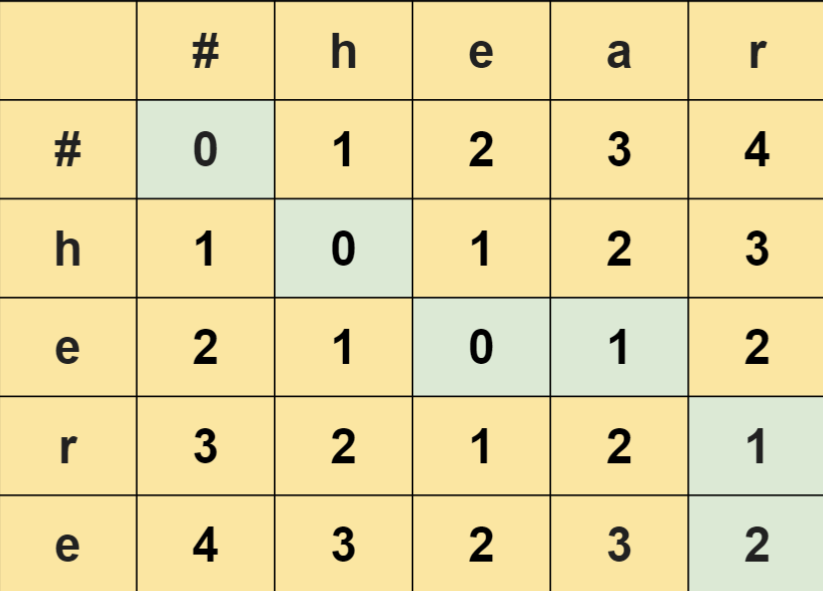
\includegraphics[width=0.5\linewidth]{LevenshteinDistance.png}
  row $i$ column $j$ = the number of operations required from
  convert first $i$ characters of source to first $j$ characters of target.

  \textbf{1.} the top left cell: 0 operations
  \textbf{2.} top row/first column: increment by $1$ because it takes
  $n$ inserts
  \textbf{3.1.} if characters in row $i$ and column $j$ are the same
  character, then $= \text{c}(i -1, j - 1)$
  \textbf{3.2.} otherwise $= 1 + \min( c(i, j - 1), c(i, j - 1), c(i
  - 1, j - 1))$

  \section{Text Normalization/Pre-Processing}
  \textbf{1.} Lowercasing
  \textbf{2.} True-casing
  \textbf{3.} Punctuation Removal
  \textbf{4.} Stopword (funciton words such as articles,
  prepositions, conjunctions and pronouns) Removal
  \textbf{5.} Stemming (takes the stem of the word - hacky e.g.
  policy and police become the same word)
  \textbf{6.} Lemmatization (map all morphologically equivalent words)

  \section{N-Gram Language Model}
  $P(w | h)  = \prod_{k = 1}^nP(w_k | w_{1 : k - 1})$
  This solution suffers from \textbf{Data Sparsity}. The exact
  history $h$ might not be present in the dataset we're using.
  Instead we can use the \textbf{Markov Assumption} and consider only
  the $N$ prior words in the past.

  \subsection{Unigram Model}
  $\approx P(w_n)$

  \subsection{Bigram Model}
  $ \approx P(w_n | w_{n - 1})$

  \subsection{N-gram Model}
  $ \approx P(w_n | w_{n - N + 1 : n - 1})$

  \subsection{Calculating Probabilties}
  $P(w | h) = \frac{C(hw)}{C(h^\star)} = \frac{C(hw)}{C(h)}$
  where
  $C(hw)$ is the count of the history followed by the word and
  $C(h*) = C(h)$ is the count of the history followed by any word

  \textit{with Laplace (Add-One) Smoothing}
  $P^L (w | h) = \frac{C(hw) + 1}{C(h) + |V|}$

  \subsection{Text Generation}
  Chose a starting point randomly on the line of most probable n-grams.
  \textbf{Unigram model:} continue sampling words randomly
  \textbf{Bigram model:} continue sampling bigrams conditioned on
  previously generated word

  \subsection{Limitations}
  N-grams don't do well at modeling long-term dependencies b.c. we
  forget old context, and N-grams don't do well with new sequences
  with similar meaning

  \subsection{Advantages}
  A clear paradigm to introduce
  \textbf{- }training and test sets
  \textbf{- }Perplexity as a metric for evaluation
  \textbf{- }Sampling to generate sentences
  \textbf{- }Other modifications to improve the model

  \section{Naive Bayes Text Classification}

  $P(c | W) = \frac{P(W | c)P(c)}{P(W)} \approx P(W|c) P(c)$
  where $P(c)$ is the prior probability of class $c$ i.e.
  $\frac{\text{Count}(c)}{\text{Count}(D)}$, number of docs with
  class $c$ divided by count of all docs $D$

  \textbf{- }$P(W)$ we \textit{could} use a language model to get
  the probability of this sequence of words, but it doesn't change
  with respect to $c$ so it's not required to get \textbf{relative}
  probabilities between classes

  \textbf{- }$P(W | c)$ is a bit more complicated so we make the
  two following assumptions

  \subsection{Assumptions}

  \textbf{Order of the words doesn't matter: }$P(W | c) = P(w_1,
  \dots, w_n | c)$ such that the likelihood of the sequence given $c$
  uses a Bag of Words

  \textbf{Words are conditionally independent:} $P(W | c) = P(w_1,
  \dots, w_n | c) = P(w_1 | c) \cdot \dots \cdot P(w_n | c)$ such
  that the probability of observing word $A$ does not affect the
  probability of observing word $B$

  \subsection{Solution Derivation}

  $\hat{c} = \arg\max_{c \in C} P(c | W)$
  $ = \arg \max _{c \in C} P(c) \prod^{N}_{i = 1}P(w_i | c)$

  it's better to operate in log space to avoid \textbf{underflow}
  $ = \arg\max_{c \in C} \log P(c) + \sum_{i = 1}^n \log P(w_i | c)$
  this is considered a \textbf{Linear Classifier}!

  To avoid division be zero, smoothing
  $P(w_i | c) = \frac{\text{count}(w_i, c) + 1}{\sum_{w \in V}(
  \text{count}(w, c) + 1)} = \frac{\text{count}(w _i, c) +
  1}{\left(\sum_{w \in V} \text{count}(w, c)\right) + |V|}$

  % \subsection{Limitation}
  % It assumes conditional independence

  \section{Logistic Regression Text Classification}
  \subsection{Binary}
  Supervised learning method where $X$ is our TF-IDF counts, $Y \in
  \{0, 1\}$ our binary class.

  Our model is
  $P(y = 1 | x) = \sigma\left(\left(\sum_{i = 1}^n w_i x_i\right) + b\right)$
  $  = \sigma(w \cdot x + b)$
  where
  $z$ is our score i.e. $P(y = 1 | x)$,
  $w$ are our weights,
  $x$ is our features,
  $b$ is our bias,
  $\sigma$ is sigmoid function

  \subsubsection{Example}
  \resizebox{\columnwidth}{!}{
    \begin{tabular}{p{1.2cm}|p{1.2cm}|p{1.2cm}|p{1.2cm}|p{1.2cm}|p{1.2cm}|p{1.2cm}|}
      \hline
      \textbf{Variable} & x1 & x2 & x3 & x4 & x5 & x6 \\ \hline
      \textbf{Meaning} & Count positive lexicon words & Count
      negative lexicon words & "No" is in document & Count 1st/2nd
      person pronouns & "!" is in document & $\log($word count$)$ \\ \hline
      \textbf{Value} & 3 & 2 & 1 & 3 & 0 & 4.19 \\ \hline
      \textbf{Weight} & 1.2 & -4 & 2.4 & 0.1 & 3.3 & -0.3 \\ \hline
    \end{tabular}
  }
  and \textbf{Bias} = 0.1

  % Then
  % $P(y^{(i)}=1| x^{(i)}) =$ %TODO
  % $P(y^{(i)}=0| x^{(i)}) =$ %TODO

  \subsection{Multinomial}
  Represent $Y$ as One-Hot Encoding and use SoftMax to map values to
  a Probability Distribution.
  Now, we will have separate weights for each class!
  For predections, we pick the class with the highest probability.
  \subsubsection{SoftMax}
  For each element $1 \le i \le K$, $\text{softmax}(z_i) =
  \frac{e^{z_i}}{\sum_{j = 1}^K e^{z_j}}$

  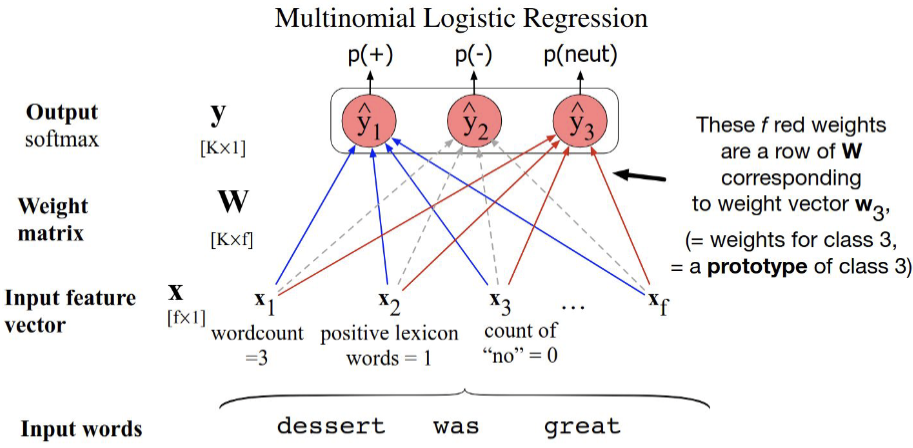
\includegraphics[width=0.48\linewidth]{MultinomialLogisticRegression.png}
  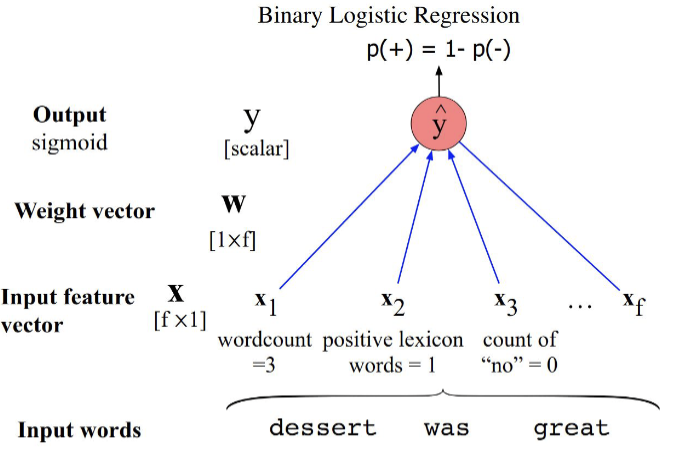
\includegraphics[width=0.48\linewidth]{BinaryLogisticRegression.png}

  \section{Neural Network}
  Our activation functions allow us to model non-linear relationships.
  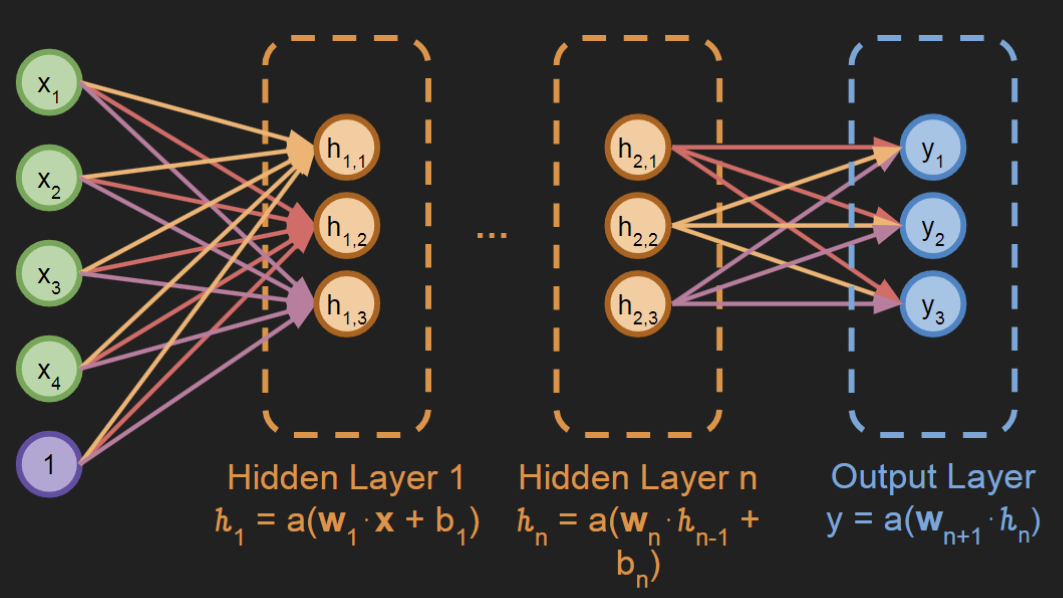
\includegraphics[width=1\linewidth]{NeuralNetwork.png}

  \subsection{Activation Functions}

  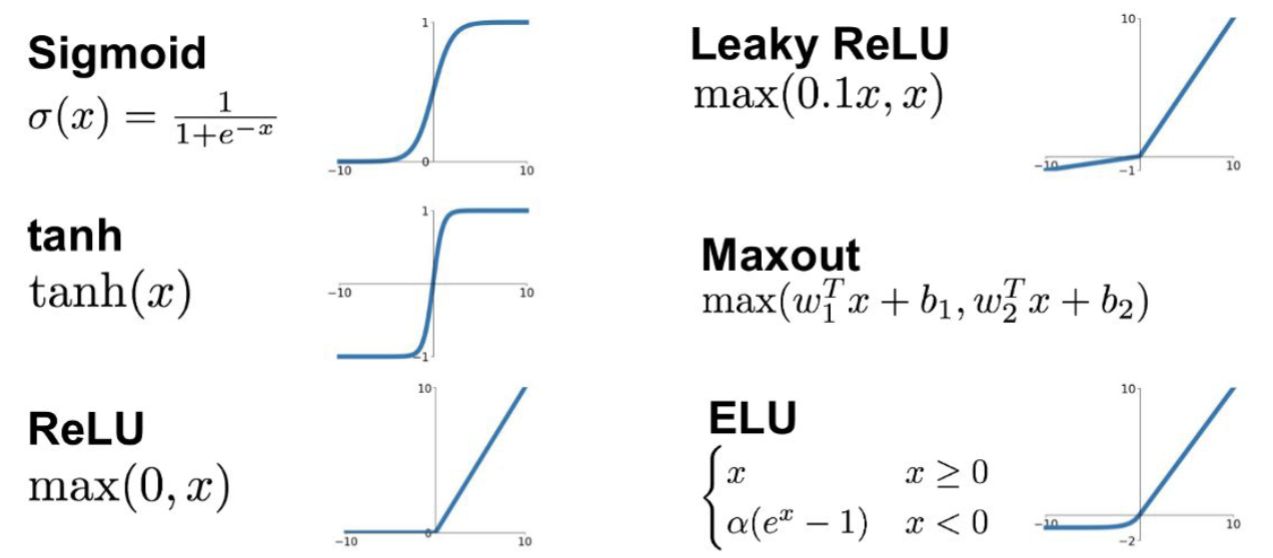
\includegraphics[width=0.45\linewidth]{ActivaitionFunctionsAndGraphs.png}
  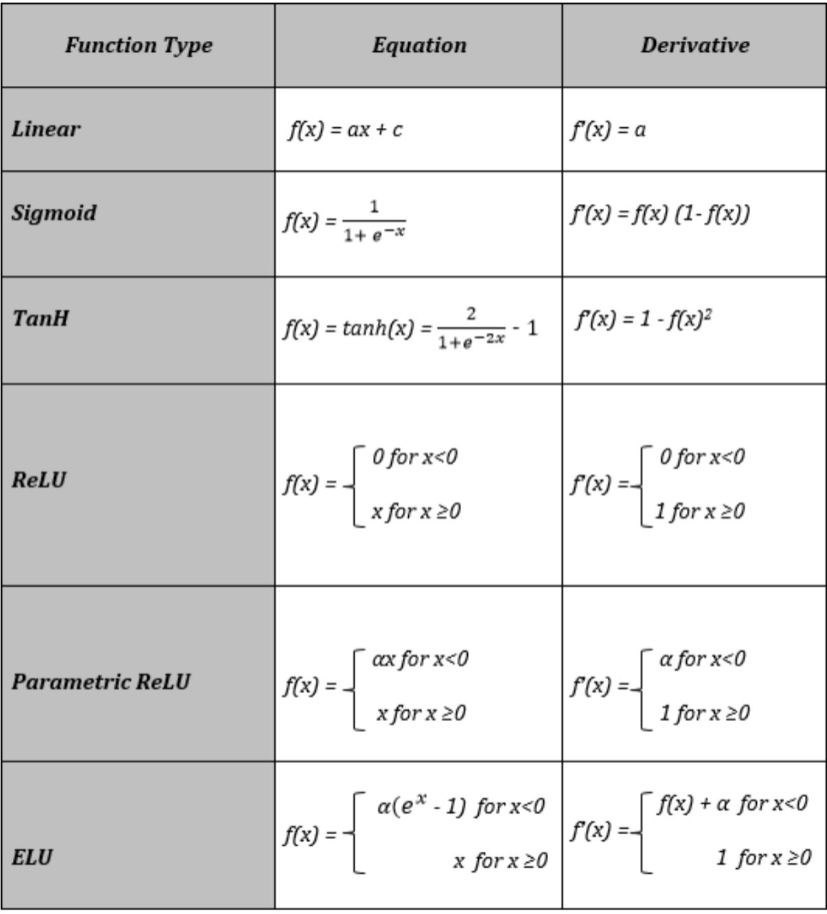
\includegraphics[width=\linewidth]{ActivationFunctionsAndDerivatives.png}

  \subsection{Backpropagation Example}
  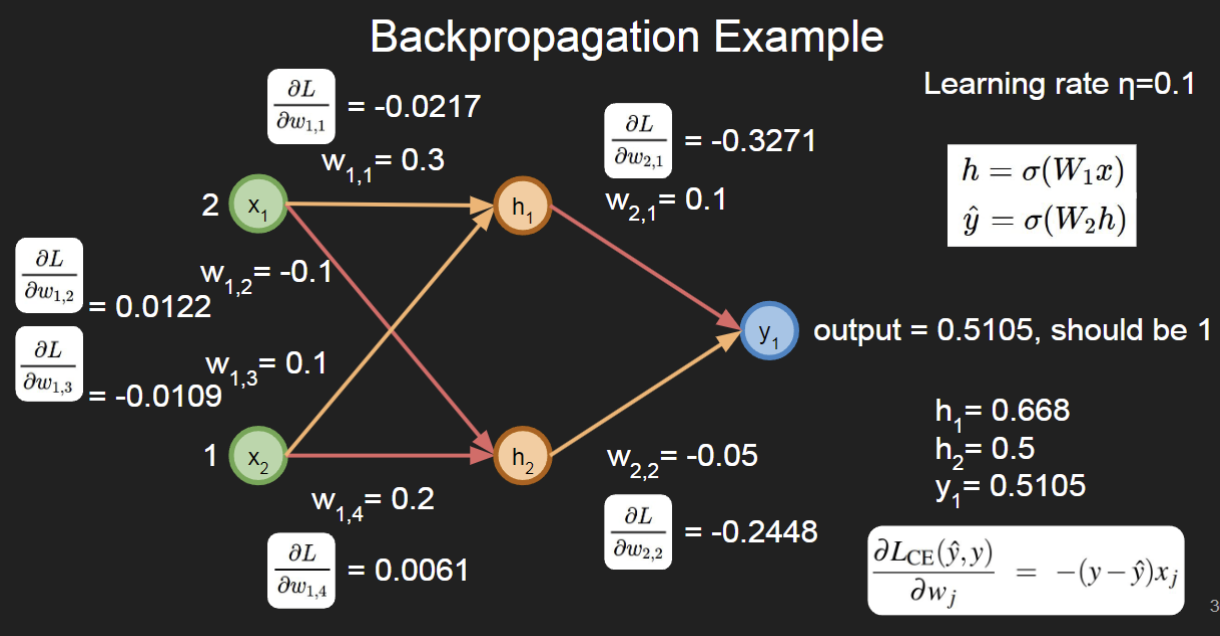
\includegraphics[width=1\linewidth]{BackpropagationExample.png}

  \section{Feature Selection}
  For example, given sentence 1 (S1) and sentence 2 (S2), does S1 entail S2?
  \textbf{1.} BLEU Score: The number of overlapping n-grams between
  two strings
  \textbf{2.} Difference in length
  \textbf{3.} Overlap of words: absolute count, percentage overlap,
  over: all words, nouns, verbs, adjectives, adverbs
  \textbf{4.} Indicator for every unigram and bigram in S2
  \textbf{5.} Count of each unigram pair between S1 and S2 that have same POS
  \textbf{6.} Count of each bigram pair between S1 and S2 that have
  the same POS in the second word

  \section{Gradient Descent}

  Let $y$ be correct label for input $x$, $\hat{y}$ be output of
  $\sigma(w \cdot x + b)$, $L(\hat{y}, y) = -[y \log \hat{y} + (1 -
  y) \log( 1 - \hat{y})]$ be the loss function (the negative log-likelihood)

  Then we update our parameters such that we find our optimal $\hat \theta$
  $\hat{\theta} = \arg \min_\theta \frac{1}{m} \sum^{m}_{i = 1}L_{CE}
  (f(x^{(i)}; \theta), y^{(i)})$
  where
  $L_{CE}$ is the loss of the true label and model prediction given
  $\theta$ and $x^{(i)}$ and
  $\frac{1}{m} \sum_{i = 1}^m$ gives the average overall points in the dataset

  \subsection{Updated a single parameter}
  $w^{t + 1} = w^t - \eta \frac{d}{dw} L(f(x; w) , y)$
  where $\eta$ is the learning rate

  \subsection{Update all parameters}
  $\theta ^{t + 1} = \theta^t - \eta \nabla L(f(x ; \theta), y)$

  % \section{Stochastic Gradient Descent}
  % %TODO add lec 11 pg 33 example

  % \section{Mini-Batch Gradient Descent}
  % %TODO

  \section{Parallelization}
  Pack everything into matrices. Modern compilers and GPUs can do
  matrix operations in parallel!!

  \section{Overfitting}
  For example, using the wrong features (e.g. model relies on the
    count of the word "Jalapenos" when trying to differentiate
    between positive and negative statements because in the corpus,
  people had good things to say about Jalapenos)

  This is what the overfitting curve looks like
  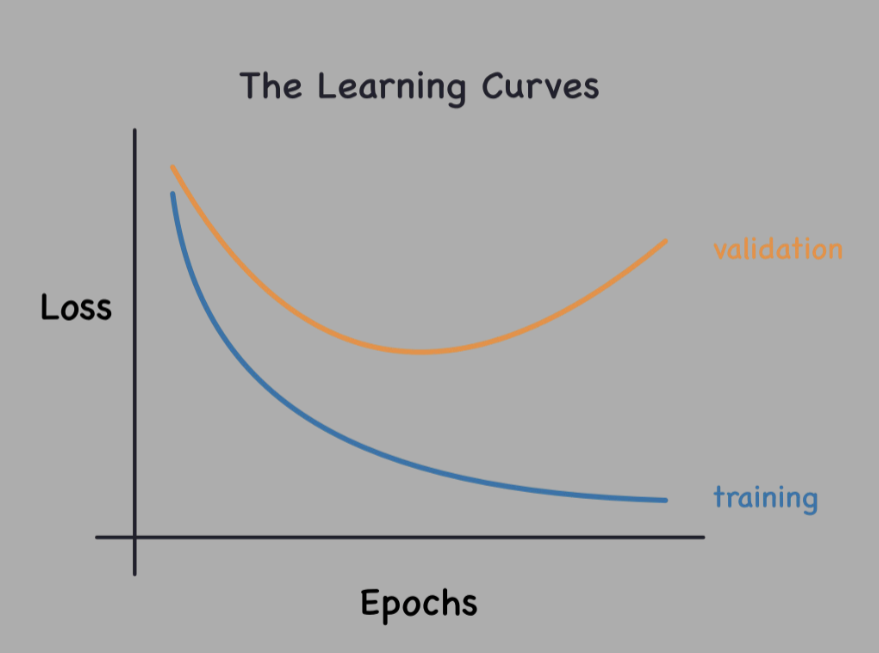
\includegraphics[width=0.5\linewidth]{Overfitting.png}

  \section{Regularization}

  \subsection{L2}
  $\hat{\theta} = \arg\max_\theta \left[\sum_{i  =1}^m \log P(y^{(i)}
  | x^{(i)})\right] - \alpha \sum_{j = 1}^n \theta^2_j $
  penalty is much higher for large values

  \subsection{L1}
  $\hat{\theta} = \arg\max_\theta \left[ \sum_{i = 1}^m \log
  P(y^{(i)} | x^{(i)}) \right] - \alpha \sum_{j = 1}^n |\theta_j|$

  \section{Hyperparameter Tuning}

  \subsection{Grid Search}
    \begin{lstlisting}
    import numpy as np
    for lr in np.linspace(0.01, 0.1, num=5):
      for bs in np.linspace(8, 32, num=4):
        # train model, eval on validation
    \end{lstlisting}
  \subsection{Random Search}
    \begin{lstlisting}
    import numpy as np
    trials = 20
    for i in range(trials):
      lr = np.random.uniform(0.01, 0.1)
      bs = np.random.randint(8, 32)
      # train model, eval on validation
    \end{lstlisting}

  \section{Cross Validation}
  \subsection{K-Fold}
  \textbf{1.} split into k equal parts
  \textbf{2.} test one part and train on the ohers
  \textbf{3.} do this for each fold
  \textbf{4.} average performance metric across all folds
  \subsection{Leave One Out}
  If you have very little data, set $K$ to the number of instances
  (e.g. train on all instances except one test on that one instance.)

  \section{Clustering}
  \subsection{K-Means}
  \textbf{1. }randomly add $k$ cluster centroids
  \textbf{2. }assign points to nearest centroid
  \textbf{3. }update the centroids based on the points
  \textbf{4. }reassign points to centroids
  \textbf{5. }move the centroids
  \textbf{6. }repeat until convergence

  \section{Jaccard Similarity}
  Similarity between phrases or sentences. Mentioning something more
  often does not matter. (It does not take into account frequency).
  $J = \frac{|A \cap B| }{|A \cup B|}$

  \section{Term Frequency Representation (TDM)}
  Each element in the vector represents the number of times the
  corresponding word appears in the document. Unlike Jaccard
  Similarity, frequency of terms plays into our similarity
  calculations. However, sometimes, stop words are a way of telling
  our models which words are important!

  \subsection{Similarity}
  \subsubsection{Euclidian Distance} $d(x_i, x_i) =
  \sqrt{\sum_{m=1}(x_{im} - x_{jm})^2}$\

  \subsubsection{Co-sine Distance}  $1 - \frac{A \cdot B}{ | A | |B
  |}$ the difference between angles

  \section{Term Frequency Inverse Document Frequency (TF-IDF)}

  \subsection{Term Frequency (TF)}
  The number of timers a term (token) appears in the document
  \resizebox{\columnwidth}{!}{
    \begin{tabular}{|l|l|}
      \hline
      Type & Description \\ \hline
      Binary & $1$ if present, else $0$ \\ \hline
      Count & Number of times it appears \\ \hline
      Frequency & $\frac{  ext{count}}{\text{total terms in
      document}}$ \\ \hline
      Log normalized count & $\log(1 + \text{count})$ \\ \hline
    \end{tabular}
  }

  \subsection{Inverse Document Frequency (IDF)}
  The inverse of term popularity in the overall corpus.
  $\text{IDF}(w, c) = \log\left(\frac{ | c| }{| d \in c : w \in d|}\right)$
  i.e. for word $w$ and corpus $c$ = for each document in the corpus,
  how many documents have the word

  \textbf{- }the intuition between the log is that at some point, if
  the word is soo frequent, we aren't really getting that much
  information by the word being repeated again
  \textbf{- }the intuition behind the denominator is that if this
  word appears in all the documents, it is not important at all

  \subsubsection{Example}
  \resizebox{0.5\columnwidth}{!}{
    \begin{tabular}{|l|l|}
      \hline
      Doc & Content \\ \hline
      1 & Jalapenos have seeds \\ \hline
      2 & Donuts are great \\ \hline
      3 & Jalapenos have flavor \\ \hline
    \end{tabular}
  }

  $\text{words} =
  \begin{bmatrix} \text{jalapenos, have, seeds, donuts, are, great, flavor}
  \end{bmatrix}$
  $\text{TF} =
  \begin{bmatrix}1 & 1 & 1 & 0 & 0 & 0 & 0
  \end{bmatrix}$
  $\text{IDF} =
  \begin{bmatrix}\log\frac{3}{2} &  \log \frac{3}{2}  & \log 3  &  0
    & 0 & 0 & 0
  \end{bmatrix}$

  \subsubsection{Limitations}

  TF-IDF still doesn't capture semantic similarity well. Our matrix
  if very sparse, which can be inefficient for memory and computation.

  \section{Latent Dirichlet Allocation (LDA)}
  Assume each document has a probability of belonging to a topic,
  each word has a probability of belonging to a topic,
  words in the same document are more likely to be in the same topic

  Let $c_t$ be the number of topics,
  $c_w$ be the number of words,
  $z$ the word by document array (randomly initialized topics),
  $n_d$ doc by topic matrix of counts,
  $n_w$ topic by word matrix of counts,
  $n_t$ vector of counts by topics

    \begin{lstlisting}
    repeat N times:
        for each word w in document d:
            remove w's topic z[d][w] from nd, nw, nt
            pz = \frac{nw[:,w] + \beta}{nt + cw \times \beta} * \frac{nd[d,:] + \alpha}{\text{len}(d) + ct \times a}
            p = pz \times \text{sum}()
            new topic z[d][w] sampled from pz
            add count for new topic back to nd, nw, nt
    \end{lstlisting}

  where $\beta$ is Laplace Smoothing over words, $\alpha$ is Laplace
  Smoothing over topics, $\frac{n_w[:, w]}{n_t}$ is the count of
  words in a topic over the number of words in a topic,
  $\frac{n_d[d,:]}{\text{len}(d)}$ is the count of words in a
  document over the number of words in a document

  \subsection{Classification Evaluation}
  \subsubsection{Accuracy}
  $\frac{TP + TN}{P + N}$

  \subsubsection{Precision}
  $\frac{TP}{TP + FP}$

  \subsubsection{Macro Precision}
  The average precision amongst all $N$ classes $c_1, \dots, c_n$
  $\frac{1}{N}\sum\text{Precision}(c_i)$

  \subsubsection{Recall}
  $\frac{TP}{TP + FN}$

  \subsubsection{Macro Recall}
  The average recall amongst all $N$ classes $c_1, \dots, c_n$
  $\frac{1}{N}\sum\text{Recall}(c_i)$

  \subsubsection{F1 Score}
  $ = 2 \times \frac{\text{Precision} \cdot
  \text{Recall}}{\text{Precision} + \text{Recall}}$

  \section{Comparing Classifiers}
  Assume Null Hypothesis/H0 (both of our models come from the *same*
  distribution) is true and determine the range of probable results.
  Compute probability that the actual (observed) result is in that
  range. If low, there is evidence to reject H0 in favor of H1.

  Using a \textbf{T-Test} would require many samples and assumes we
  are working with a normal distribution.

  \subsection{Non-Parametric Tests}

  \subsubsection{Bootstrapped}
  sample with replacement

  Let $s$ be the number of times the difference of new test set is
  $\ge 0$ i.e.
  $s = \delta(x_i) - \delta (x) \ge 0$
  the number of times we sampled a difference at least as large as
  the observed difference

  The $p$-value is defined as
  $p = \frac{s}{b}$
  i.e. the probability of an observation at least as large as the
  observed one is happening under the H0 (where H0 = $B$ is actually
  not better than $A$, in general).

  However, we are sampling from our test set which does not have mean
  $0$. The mean is $\delta(x)$, so instead we should check
  $\delta(x_i) - \delta(x) \ge \delta(x)$
  $\Rightarrow \delta(x_i) \ge 2 \delta(x)$

  % \subsubsection{Pairwise}
  % %#todo missing

  \section{Language Model Evaluation}
  \subsection{Perplexity}
  It's the inverse of the probability that the model assigns to the
  held out data (lower is better).
  Shows what is the probability that it will be in the right bin

  $\text{Perplexity}(W) = P(w_1w_2\dots w_n)^{ - \frac{1}{N}} =
  \sqrt[N]{\frac{1}{P(w_1w_2\dots w_n)}}$

  \subsubsection{N-Gram}
  Then for an n-gram language model
  $ = \sqrt[N]{\prod^{N}_{i = 1}\frac{1}{P(w_i | w_1\dots w_{i  - 1})}}$
  $ = e^{\frac{1}{N} \sum_{i = 1}^N - \log(P(w_i | w_1 \dots w_{i -1}))}$

  \subsubsection{Unigram}
  $ = \sqrt[N]{\prod_{i = 1}^N \frac{1}{P(w_i)}}$
  \subsubsection{Bigram}
  $ = \sqrt[N]{\prod_{i = 1}^N \frac{1}{P(w_i | w_{i - 1})}}$

  \section{Topic Model Evaluation: Intrusion Methods}
  Using, for example, Amazon mechanical Turk
  \subsubsection{Word Intrusion}
  Are topics meaningful, interpretable, coherent, useful?
  \textbf{e.g.} take the highest probability words from a topic, take
  a high-probability word form another topic and add it,
  \textit{hypothesis} if the topics are interpretable, users with
  consistency choose the correct intruder

  \subsubsection{Topic Intrusion}
  Is assignment of topics to documents meaningful, appropriate, useful?
  \textbf{e.g} display document title and first 500 characters, show
  the three topics with highest probability and one topic chosen
  randomly, have the user click on the set of words that is out of
  place, \textit{hypothesis} if the association of topics to a
  document is interpretable, users with consistently choose the true
  intruding topic

  \subsection{Topic Coherence (Umass Version)}
  $C(t; V^{(t)}) = \sum^{M}_{m = 2} \sum_{l = 1}^{m -1} \log
  \frac{D(v_m^{(t)}, v_l^{(t)}) + 1}{D(v_t^{(t)})} $
  where $C(t; V(t))$ is the coherence of topic $t$ given $V(t)$, the
  $M$ most probable words in $t$,
  $D(v)$ how many documents contain word $v$,
  $D(v, v')$ how many documents contain both words (co-document frequency)

  % studies show coherence tends to correlate with topic intrusion
  % correct guesses

  \section{Discriminative vs Generative}
  \resizebox{\columnwidth}{!}{
    \begin{tabular}{|l|p{2.5cm}|p{2.5cm}|}
      \hline
      Method & Generative & Discriminative \\ \hline
      Learns & Estimate $P(x \| y)$ to then deduce $P(y \| x)$ &
      Directly estimate $P(y \| x)$ \\ \hline
    \end{tabular}
  }

  \section{Q\&A}
  \scriptsize

  \question{the set of all alphabetic strings}
  \answer{[a-zA-Z]+}

  \question{the set of all lower case alphabetic strings ending in a b}
  \answer{\textbackslash b[a-z]*b\textbackslash b}

  \question{the set of all strings from the alphabet a, b such that
  each a is immediately preceded by and immediately followed by a b}
  \answer{\textbackslash b b+ (ab+)+ \textbackslash b}

  \question{the set of all strings with two consecutive repeated
    words (e.g., "Humbert Humbert" and "the the" but not "the bug" or
  "the big bug")}
  \answer{(.+)\textbackslash b \textbackslash 1}

  \question{all strings that start at the beginning of the line with
  an integer and that end at the end of the line with a word}
  \answer{\textasciicircum [0-9]+.*[A-Za-z]+\$}

  \question{all strings that have both the word grotto and the word
    raven in them (but not, e.g., words like grottos that merely
  contain the word grotto)}
  \answer{\textbackslash b grotto \textbackslash b .* \textbackslash
    b raven \textbackslash b \vline \textbackslash b raven
  \textbackslash b .* \textbackslash b grotto \textbackslash b}

  \question{
    ELIZA-like program
  }

    \begin{lstlisting}
    s/.* YOU ARE (depressed|sad) .*/I AM SORRY TO HEAR YOU ARE \1/ s/.*
    YOU ARE (depressed|sad) .*/WHY DO YOU THINK YOU ARE \1/ s/.*
    all .*/IN WHAT WAY/ s/.*
    always .*/CAN YOU THINK OF A SPECIFIC EXAMPLE/
    \end{lstlisting}

  \question{
    Edit distance of “leda” to “deal”.
  }

  \answer{
    \resizebox{0.4\columnwidth}{!}{
      \begin{tabular}{|l|l|l|l|l|l|}
        \hline
        &   & D & E & A & L \\ \hline
        ~ & 0 & 1 & 2 & 3 & 4 \\ \hline
        L & 1 & 1 & 2 & 3 & 3 \\ \hline
        E & 2 & 2 & 1 & 2 & 3 \\ \hline
        D & 3 & 2 & 2 & 2 & 3 \\ \hline
        A & 4 & 3 & 3 & 2 & 3 \\ \hline
      \end{tabular}
    }
  }

  \question{
    All the non-zero trigram probabilities.
  }

    \begin{verbatim}
    <s> I am Sam </s>
    <s> Sam I am </s>
    <s> I do not like green eggs and ham </s>
    \end{verbatim}

  $P(w_n | w_{n-2} w_{n-1}) = \frac{C(w_{n-2}, w_{n-1},
  w_n)}{C(w_{n-2}, w_{n-1})}$

  $P(\text{am} | \langle s \rangle,  I) = \frac{1}{2}$
  $P(\text{Sam} | \text{I}, \text{am}) = \frac{1}{2}$

  \question{
    probability of \texttt{i want chinese food}. One using regular
    table, another using the add-1 smoothed table.
  }

  $P(\text{i want chinese food}) = P(\text{i} | ) P(\text{want} |
  \text{i}) P(\text{chinese} | \text{want}) P(\text{food} |
  \text{chinese}) P( \langle  / s \rangle | \text{food}) = 0.0001896$
  using add-1 smoothing $= 0.000002406$

  \question{
    Which is higher? Why?
  }

  Unsmoothed is higher because the bigrams used in the sentence are
  common in the corpus. However, with add-1 smoothing, the
  probability mass is redistributed to account for unseen n-grams,
  reducing the probabilities of frequent bigrams.

  \question{
    Using a bigram language model with add-one smoothing, what is \(
    P(\text{Sam} | \text{am}) \)?
  }

    \begin{verbatim}
    add <s> I am Sam </s> to line 3
    \end{verbatim}

  $P(\text{Sam} | \text{am}) = \frac{C(am, \text{Sam}) + 1}{C(\text{am}) + V}$
  $= \frac{2 + 1}{3 + 11}$
  $= 0.214$

  \vspace{3px}
  \question{

    \begin{multicols}{2}
      What class will Naive Bayes assign to the sentence “I always
      like foreign films.”?
      (assume equal prior probabilities for each class)

      \begin{tabular}{|c|c|c|}
        \hline
        Word & Pos & Neg \\
        \hline
        I & 0.09 & 0.16 \\
        always & 0.07 & 0.06 \\
        like & 0.29 & 0.06 \\
        foreign & 0.04 & 0.15 \\
        films & 0.08 & 0.11 \\
        \hline
      \end{tabular}
    \end{multicols}
  }

  For positive
  $P(s | \text{pos}) $
  $= P(\text{I} | \text{pos}) P(\text{always} | \text{pos})$
  $ P(\text{like} | \text{pos}) P(\text{foreign} | \text{pos})$
  $ P(\text{films} | \text{pos})$
  $= 0.09 \times 0.07 \times 0.29 \times 0.04 \times 0.08$
  $= 0.00005846$

  For negative

  $P(s | \text{neg}) $
  $= P(I | \text{neg}) P(\text{always} | \text{neg}) $
  $P(\text{like} | \text{neg}) P(\text{foreign} | \text{neg}) $
  $P(\text{films} | \text{neg})$
  $= 0.16 \times 0.06 \times 0.06 \times 0.15 \times 0.11$
  $= 0.00009504$

  Since
  $P(s | \text{neg}) > P(s | \text{pos})$

  the Naive Bayes classifier assigns the negative class to the sentence.

  \question{
    \begin{multicols}{2}

      Compute the most likely class for

      \textbf{"fast, coup, shoot, fly"}

      Assume a naive Bayes and add-1 smoothing.

      \begin{tabular}{|l|l|}
        \hline
        Rev. & Cat. \\
        \hline
        fun, coup, love, love & com  \\
        fast, fur, shoot & act \\
        coup, fly, fast, fun & com  \\
        fur, shoot, shoot, fun & act  \\
        fly, fast, shoot, love & act  \\
        \hline
      \end{tabular}
    \end{multicols}
  }

  First, priors
  $P(\text{com}) = \frac{2}{5} = 0.4$,$ P(\text{act}) = \frac{3}{5} = 0.6$

  Vocab size
  $|V| = 7$

  Likelihoods for each word where
  $P(w | \text{class}) = \frac{C(w, \text{class}) + 1}{\sum C(w,
  \text{class}) + |V|}$

  \textbf{Computed Likelihoods:}

  $P(\text{fast} | \text{com}) = \frac{1+1}{9+7} = \frac{2}{16}$,$
  P(\text{fast} | \text{act}) = \frac{2+1}{11+7} = \frac{3}{18}$

  $P(\text{coup} | \text{com}) = \frac{2+1}{9+7} =
  \frac{3}{16}$,$P(\text{coup} | \text{act}) = \frac{0+1}{11+7} = \frac{1}{18}$

  $P(\text{shoot} | \text{com}) = \frac{0+1}{9+7} =
  \frac{1}{16}$,$P(\text{shoot} | \text{act}) = \frac{4+1}{11+7} = \frac{5}{18}$

  $P(\text{fly} | \text{com}) = \frac{1+1}{9+7} =
  \frac{2}{16}$,$P(\text{fly} | \text{act}) = \frac{1+1}{11+7} = \frac{2}{18}$

  Using Naive Bayes assumption:

  $P(D | \text{com}) = P(\text{fast} | \text{com}) $
  P(\text{coup} | \text{com}) P(\text{shoot} | \text{com}) $
  P(\text{fly} | \text{com}) P(\text{com})$
  $= \frac{2}{16} \times \frac{3}{16} \times \frac{1}{16} \times
  \frac{2}{16} \times \frac{2}{5}$
  $= 0.000073242$

  $P(D | \text{act}) = P(\text{fast} | \text{act}) $$
  P(\text{coup} | \text{act}) P(\text{shoot} | \text{act})$
  $ P(\text{fly} | \text{act}) P(\text{act})$
  $= \frac{3}{18} \times \frac{1}{18} \times \frac{5}{18} \times
  \frac{2}{18} \times \frac{3}{5}$
  $= 0.000171468$

  Since $P(D | \text{act}) > P(D | \text{com})$ the document \(D\) is
  classified as act

  \question{

    Train two models, multinomial vs binary naive Bayes, both with
    add-1 smoothing.

    Classify "\textbf{A good, good plot and great characters, but poor acting.}"

    Do the two models agree or disagree?

    \begin{tabular}{|c|c|c|c|c|}
      \hline
      Doc & “Good” & “Poor” & “Great” & Class \\
      \hline
      d1 & 3 & 0 & 3 & pos \\
      d2 & 0 & 1 & 2 & pos \\
      d3 & 1 & 3 & 0 & neg \\
      d4 & 0 & 2 & 0 & neg \\
      d5 & 0 & 2 & 0 & neg \\
      \hline
    \end{tabular}

  }

  Priors
  $P(\text{pos}) = \frac{2}{4} = 0.5$,$P(\text{neg}) = \frac{2}{4} = 0.5$

  Vocab $|V| = 3$

  \textbf{Likelihoods}
  $P(w | \text{class}) = \frac{C(w, \text{class}) + 1}{\sum C(w,
  \text{class}) + |V|}$

  $P(\text{good} | \text{pos}) = \frac{3+1}{9+3} = \frac{4}{12},
  \quad P(\text{good} | \text{neg}) = \frac{2+1}{14+3} = \frac{3}{17}$

  $P(\text{poor} | \text{pos}) = \frac{1+1}{9+3} = \frac{2}{12},
  \quad P(\text{poor} | \text{neg}) = \frac{10+1}{14+3} = \frac{11}{17}$

  $P(\text{great} | \text{pos}) = \frac{5+1}{9+3} = \frac{6}{12},
  \quad P(\text{great} | \text{neg}) = \frac{2+1}{14+3} = \frac{3}{17}$

  \textbf{Multinomial:}
  $P(D | \text{pos}) = P(\text{good} | \text{pos})^2 P(\text{poor} |
  \text{pos}) P(\text{great} | \text{pos}) P(\text{pos})$
  $= \left(\frac{4}{12}\right)^2 \times \frac{2}{12} \times
  \frac{6}{12} \times 0.5$
  $= 0.000055$

  For negative
  $P(D | \text{neg}) = P(\text{good} | \text{neg})^2 P(\text{poor} |
  \text{neg}) P(\text{great} | \text{neg}) P(\text{neg})$
  $= \left(\frac{3}{17}\right)^2 \times \frac{11}{17} \times
  \frac{3}{17} \times 0.5$
  $= 0.00014$

  since
  $
  P(D | \text{neg}) > P(D | \text{pos})
  $
  the document \(D\) is classified as negative

  \textbf{Binarized}
  $P(D | \text{pos}) = P(\text{good} | \text{pos}) P(\text{poor} |
  \text{pos}) P(\text{great} | \text{pos}) P(\text{pos})$
  $= \frac{2}{7} \times \frac{3}{7} \times \frac{2}{7} \times 0.5$
  $= 0.0139$

  $P(D | \text{neg}) = P(\text{good} | \text{neg}) P(\text{poor} |
  \text{neg}) P(\text{great} | \text{neg}) P(\text{neg})$
  $= \frac{3}{9} \times \frac{2}{9} \times \frac{4}{9} \times 0.5$
  $= 0.0197$

  Since
  $P(D | \text{neg}) > P(D | \text{pos})$

  Therefore,  both models classify the document as negative, meaning
  they agree on the classification.

  \section{Credits}
  \begin{itemize}
    \item Sarah for initial Overleaf version
  \end{itemize}
\end{multicols*}

\end{document}
